\documentclass{standalone}
\usepackage{tikz}
\usepackage{emoji}
\usetikzlibrary{positioning,arrows.meta,shapes.misc,calc}

% COLORS
\usepackage{xcolor}
\colorlet{myred}{red!80!black}
\colorlet{myblue}{blue!80!black}
\colorlet{mybluee}{myblue!80!black}
\colorlet{mygreen}{green!60!black}
\colorlet{myorange}{orange!70!red!60!black}
\colorlet{mydarkred}{red!30!black}
\colorlet{mydarkblue}{blue!40!black}
\colorlet{mydarkgreen}{green!30!black}

\begin{document}
\begin{tikzpicture}[
    >=Stealth,
    block/.style={rectangle, rounded corners, draw, minimum width=2cm, minimum height=1cm, align=center},
]

% Input block
\node[draw=black, rounded corners, thick, minimum width=3.8cm, minimum height=2.3cm, xshift=-1.2cm, yshift=-0.4cm] (input) at (5.9,-3.7) {
    \begin{minipage}{2cm}
        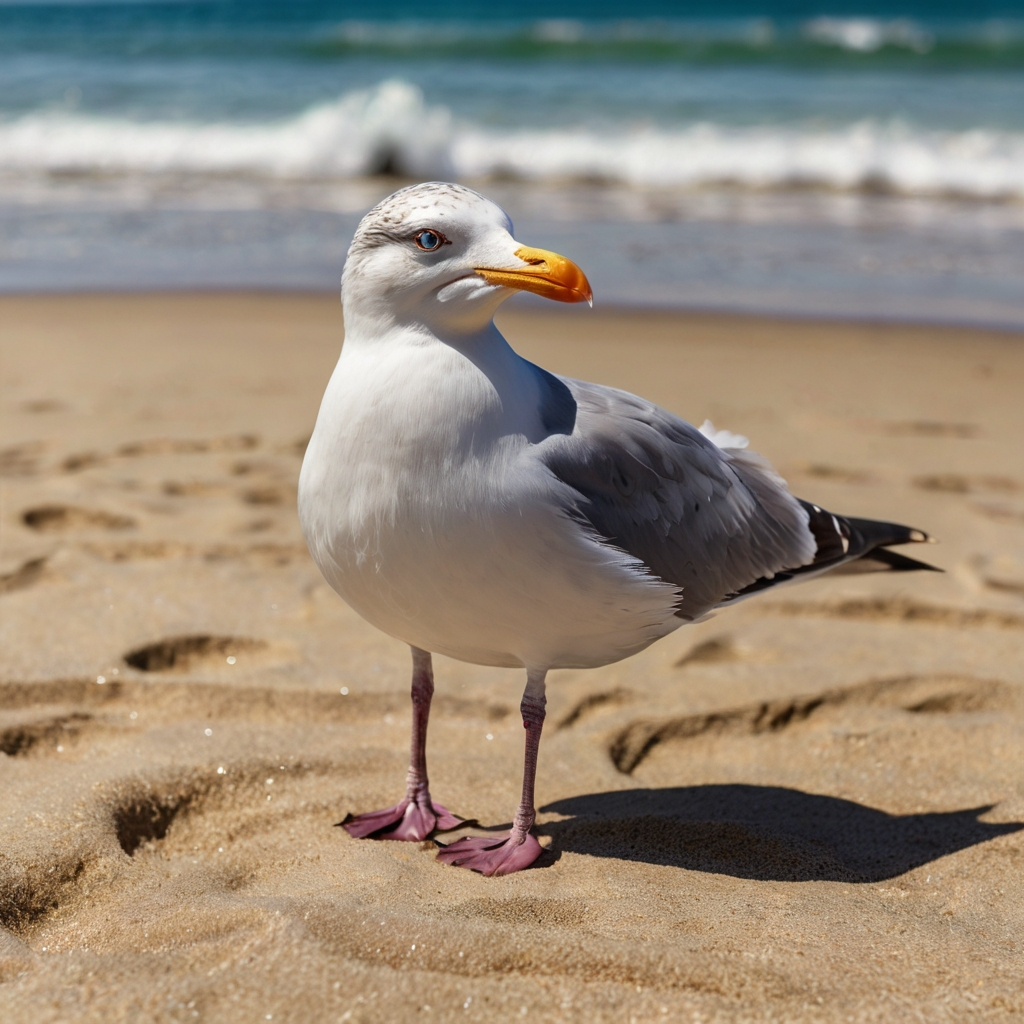
\includegraphics[width=2cm,height=2cm]{images/seagull.jpg} 
    \end{minipage}%
    \hspace{0.3cm}%
    \begin{minipage}{2cm}
        \centering
        a seagull is chilling \\
        (\emoji{smiling-face-with-sunglasses}) on the beach
    \end{minipage}
};

% Main components on the same line
\node[block, black, draw=black,fill=mygreen!20] (encoder) at (0,0) {Image\\Encoder};
\node[block, black,draw=black,fill=myblue!20, right=2cm of encoder] (llm) {LLM for Language \\ Understanding and \\ Generation};
\node[block, black, draw=black,fill=myred!20, right=2cm of llm] (generator) {Image\\Generation};

% Arrows and labels
\draw[->] (encoder) -- node[above, align=center] {} (llm);
\draw[->] (llm) -- node[above, align=center] {} (generator);

% Additional text
\node[text width=3cm, below=0.2cm of generator, align=center] {Produce \\ Visual Data};
\node[text width=3cm, below=0.2cm of encoder, align=center] {Consume \\ Visual Data};
\node[above=0.25cm of input] {Example of Input Data: (Image + Text)};

\end{tikzpicture}
\end{document}